\documentclass[a4paper,12pt]{article}
\usepackage[utf8]{inputenc}
\usepackage[bulgarian]{babel}
\usepackage{hyperref}
\usepackage{listings}
\usepackage{xcolor}
\usepackage{graphicx}
\usepackage{geometry}
\geometry{margin=1in}

% Код формат
\lstset{
    basicstyle=\ttfamily\footnotesize,
    breaklines=true,
    backgroundcolor=\color{gray!10},
    frame=single
}

\title{Документация на проекта за управление на полети и самолети}
\author{}
\date{\today}

\begin{document}

\maketitle

\tableofcontents
\newpage

\section{Въведение}
Проектът е разработен с цел да подпомогне авиокомпании при управлението на ресурси чрез оптимизиране на самолетните полети. 
Целите на проекта включват:
\begin{itemize}
    \item Съхранение на информация за самолети и полети.
    \item Извършване на търсения за съвместимост между самолети и дестинации.
    \item Оценка на ефективността и ресурсоемкостта на даден самолетен маршрут.
\end{itemize}

\section{Файлова структура}
Проектът съдържа следните основни файлове:
\begin{itemize}
    \item \texttt{main.cpp}: Основният файл за изпълнение.
    \item \texttt{airport.cpp}, \texttt{airport.hpp}: Модул за управление на летища.
    \item \texttt{airspace\_manager.cpp}, \texttt{airspace\_manager.hpp}: Логика за управление на въздушното пространство.
    \item \texttt{plane.cpp}, \texttt{plane.hpp}: Информация и операции, свързани със самолети.
    \item \texttt{flight.cpp}, \texttt{flight.hpp}: Управление на полети.
    \item \texttt{date\_time.cpp}, \texttt{date\_time.hpp}: Помощни функции за работа с дата и час.
    \item \texttt{enumerable.cpp}, \texttt{enumerable.hpp}: Общи структури за работа с итерации.
    \item \texttt{CMakeLists.txt}: Конфигурация на проекта.
    \item \texttt{Doxyfile}: Настройки за генериране на документация чрез Doxygen.
    \item \texttt{description.txt}: Текстово описание на проекта.
\end{itemize}

\section{Описание на модулите}
\subsection{Модул \texttt{Plane}}
Модулът управлява информацията за самолетите. Той съдържа следния клас:

\subsubsection*{Клас \texttt{Plane}}
\textbf{Полетата на класа:}
\begin{itemize}
    \item \texttt{std::string id}: Идентификационен номер на самолета.
    \item \texttt{std::string manufacturer}: Производител на самолета.
    \item \texttt{std::string model}: Модел на самолета.
    \item \texttt{int seats}: Брой седалки.
    \item \texttt{double runway\_length}: Минимална дължина на пистата за кацане.
    \item \texttt{double fuel\_consumption}: Разход на гориво за 1 км на място.
    \item \texttt{double tank\_capacity}: Обем на резервоара.
    \item \texttt{double average\_speed}: Средна скорост.
\end{itemize}

\paragraph*{Член-функции:}
\begin{itemize}
    \item \texttt{Plane(const std::string\&, const std::string\&, const std::string\&, int, double)}: Конструктор за инициализация.
    \item \texttt{void setId(const std::string\&)}: Задава идентификационен номер.
    \item \texttt{std::string getId() const}: Връща идентификационния номер.
    \item \texttt{void printDetails() const}: Извежда информация за самолета.
    \item \texttt{bool canReachDestination(double distance, double runway) const}: Проверява съвместимостта с дадена дестинация.
\end{itemize}

\subsection{Модул \texttt{Flight}}
Модулът управлява полетите. Той съдържа следния клас:

\subsubsection*{Клас \texttt{Flight}}
\textbf{Полетата на класа:}
\begin{itemize}
    \item \texttt{std::string flight\_id}: Идентификатор на полета.
    \item \texttt{std::string destination}: Дестинация.
    \item \texttt{double distance}: Разстояние на полета.
    \item \texttt{Plane assigned\_plane}: Назначен самолет.
\end{itemize}

\paragraph*{Член-функции:}
\begin{itemize}
    \item \texttt{Flight(const std::string\&, const std::string\&, double)}: Конструктор за инициализация.
    \item \texttt{void assignPlane(const Plane\&)}: Назначава самолет към полета.
    \item \texttt{bool isCompatible(const Plane\&) const}: Проверява дали самолетът е съвместим с полета.
    \item \texttt{void printFlightDetails() const}: Извежда информация за полета.
\end{itemize}

\subsection{Модул \texttt{AirspaceManager}}
Модулът управлява съвместимостта между самолети и дестинации. Той съдържа следния клас:

\subsubsection*{Клас \texttt{AirspaceManager}}
\textbf{Полетата на класа:}
\begin{itemize}
    \item \texttt{std::vector<Plane> planes}: Списък със самолети.
    \item \texttt{std::vector<Flight> flights}: Списък с полети.
\end{itemize}

\paragraph*{Член-функции:}
\begin{itemize}
    \item \texttt{void addPlane(const Plane\&)}: Добавя самолет към списъка.
    \item \texttt{void addFlight(const Flight\&)}: Добавя полет към списъка.
    \item \texttt{std::vector<Plane> findCompatiblePlanes(const Flight\&) const}: Връща списък с подходящи самолети за даден полет.
    \item \texttt{void printAllFlights() const}: Извежда информация за всички полети.
    \item \texttt{void printAllPlanes() const}: Извежда информация за всички самолети.
\end{itemize}

\subsection{Модул \texttt{DateTime}}
Модул за управление на дата и час. Той съдържа следния клас:

\subsubsection*{Клас \texttt{DateTime}}
\textbf{Полетата на класа:}
\begin{itemize}
    \item \texttt{int year, month, day, hour, minute, second}: Компоненти на дата и час.
\end{itemize}

\paragraph*{Член-функции:}
\begin{itemize}
    \item \texttt{DateTime(int, int, int, int, int, int)}: Конструктор за инициализация.
    \item \texttt{std::string toString() const}: Връща датата и часа като текст.
    \item \texttt{bool isBefore(const DateTime\&) const}: Проверява дали една дата предхожда друга.
\end{itemize}

\section{UML Диаграма}
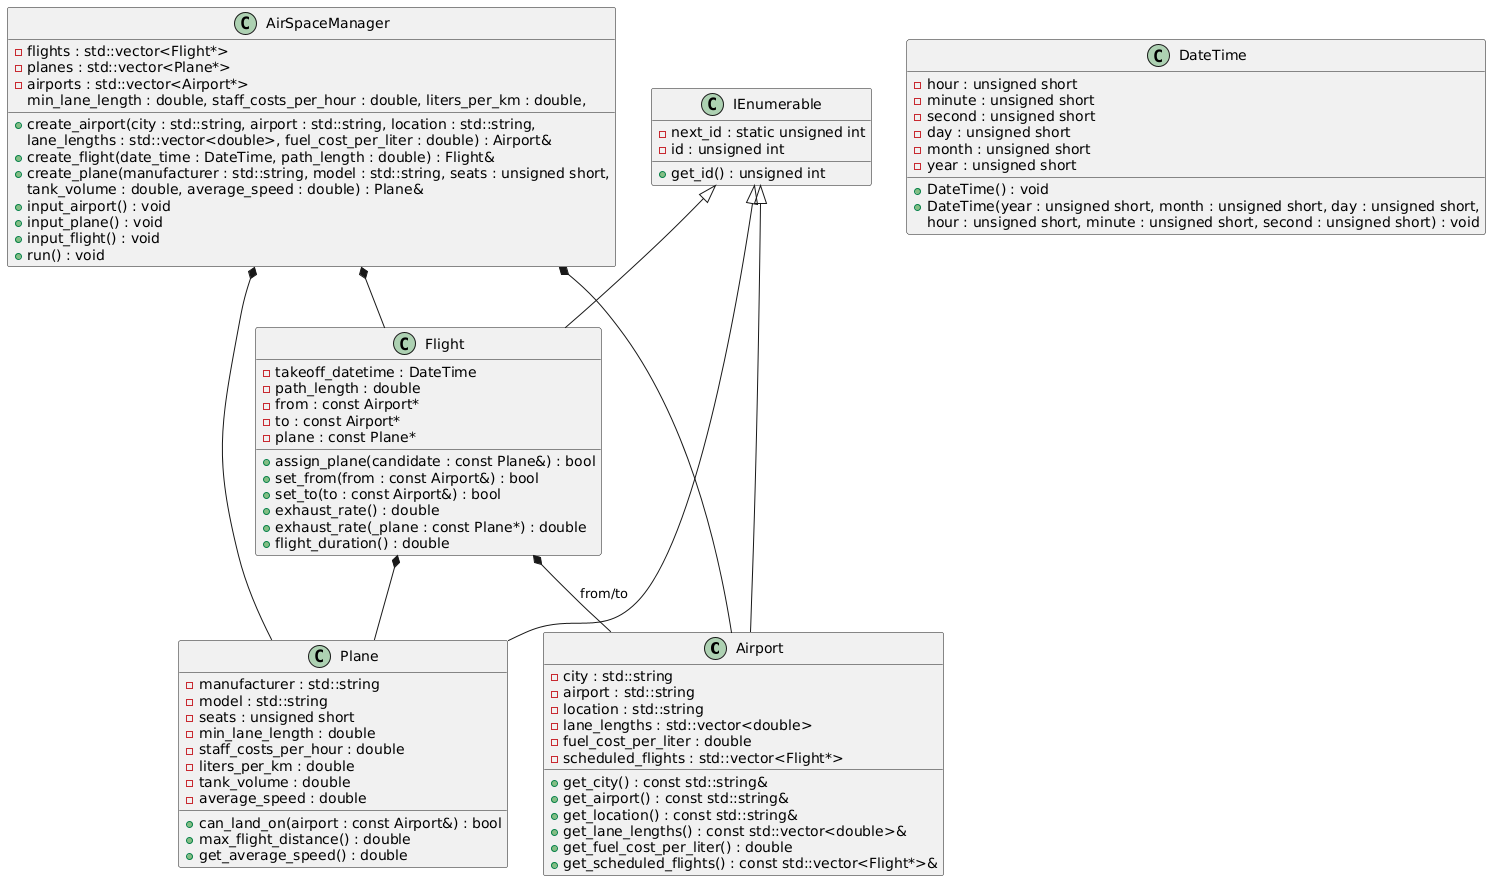
\includegraphics[width=\textwidth]{uml_diagram.jpg} % Вмъкнете вашата UML диаграма тук.

\end{document}
